\documentclass{article}


% load package with some of the available options - you may not need this!
\usepackage[framed,autolinebreaks,useliterate]{mcode}

% for checklist
\usepackage{enumitem,amssymb}
\newlist{todolist}{itemize}{2}
\setlist[todolist]{label=$\square$}
\usepackage{pifont}
\newcommand{\cmark}{\ding{51}}%
\newcommand{\xmark}{\ding{55}}%
\newcommand{\done}{\rlap{$\square$}{\raisebox{2pt}{\large\hspace{1pt}\cmark}}%
\hspace{-2.5pt}}
\newcommand{\wontfix}{\rlap{$\square$}{\large\hspace{1pt}\xmark}}


% something NOT relevant to the usage of the package.
\usepackage{graphicx}
\usepackage{url,textcomp}
\setlength{\parindent}{0pt}
\setlength{\parskip}{18pt}
\title{ECTA Homework 4\\Multiobjective Optimization with the\\Non-dominated Sorting Genetic Algorithm II}
\author{\color{red} Djordje Vukcevic, \texttt{djordje.vukcevic@smail.inf.h-brs.de}\\
	\color{red}	Supriya Vadiraj,\texttt{supriya.vadiraj @smail.inf.h-brs.de}}
% //////////////////////////////////////////////////

\begin{document}

\maketitle

\section{The Assignment}

\subsection{NSGA-II (75pts)}
\begin{itemize}
	\item (50pts) Implement NSGA-II to find all non-dominated solutions to the trailing ones, leading zeros problem. 
	\begin{itemize}
		\item Bitstring with length 20
		\item Population size of 100
		\item Generations 100
		\item Hints:
		\begin{itemize}
			\item Crossover and mutation can be performed just as in other bit string problems, e.g. one-max
			\item The \mcode{sortrows} function can be used to sort matrices, you can use this first before implementing NSGAs sorting
		\end{itemize}
	\end{itemize}
	\item (20pts) Visualize the progress of your algorithm over a single 100 generation run with an animated gif (1 frame every generation).
	\begin{itemize}
		\item Use the code here: \url{https://www.mathworks.com/matlabcentral/fileexchange/63239-gif} to create gif
		\begin{itemize}
			\item Set the timing so that the gif completes in a reasonable amount of time (between 10 and 20 seconds)
		\end{itemize}
		\item Fronts can be visualized with the code snippets attached\\ (\mcode{displayFronts.m})
	\end{itemize}
	\item (5pts) At each iteration mark the individuals which carry on to the next population, and which do not (you will have to code this yourself).
\end{itemize}


\subsection{Short Answer (25pts)}
\begin{itemize}
	\item (10pts) Compare the sort used by NSGA-II with a variety of population sizes. How long does 100 generations take with each approach when using a population size of:
	\begin{enumerate}
		\item 10: 1.762199 seconds
		\item 100: 173.002463 seconds
		\item 1000: 16759.334529 seconds
	\end{enumerate}
	\item (5pts) Plot the end result of a single run with [100 pop and 100 gen] and [10 pop and 1000 gen]. Describe the difference between the end results. Which is preferable?
	
		\begin{figure}[h]
			\begin{center}
				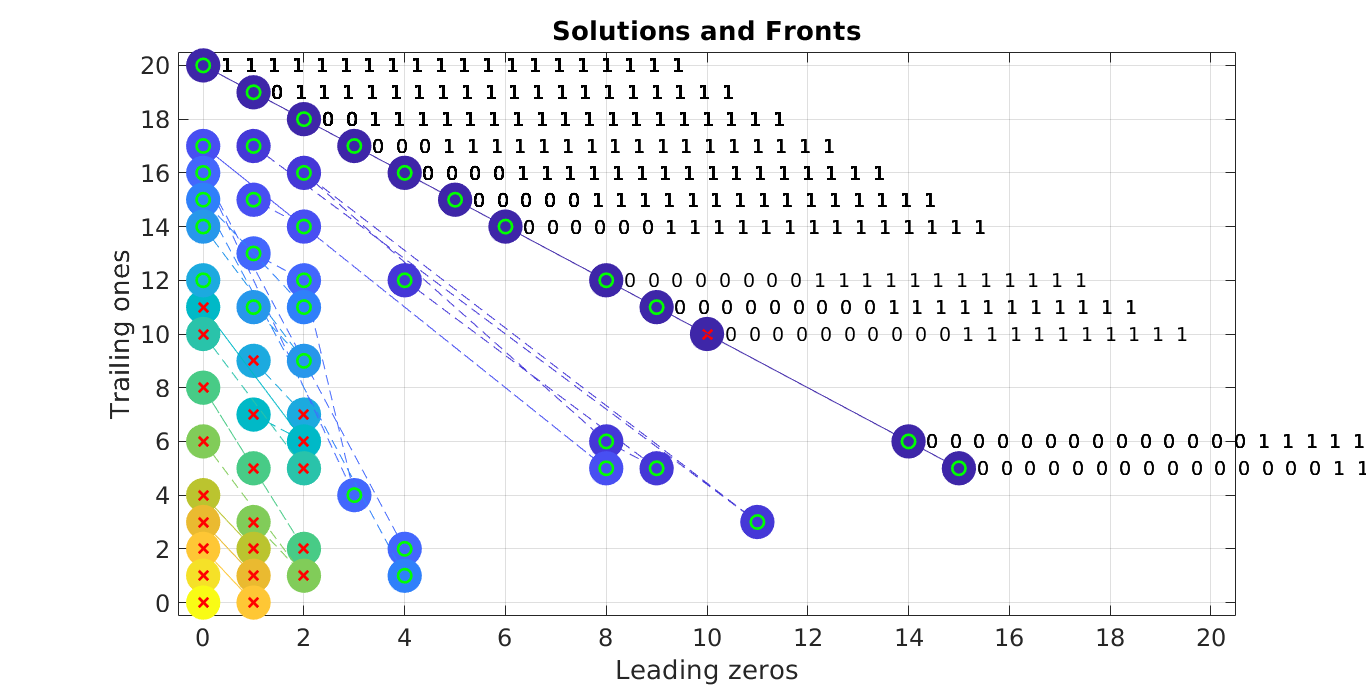
\includegraphics[width=\textwidth]{100_gen_100_pop.png}
			\end{center}
			\caption{Population size = 100, while number of generations = 100}
			\label{figure1}
		\end{figure}
		
			\begin{figure}[h]
				\begin{center}
					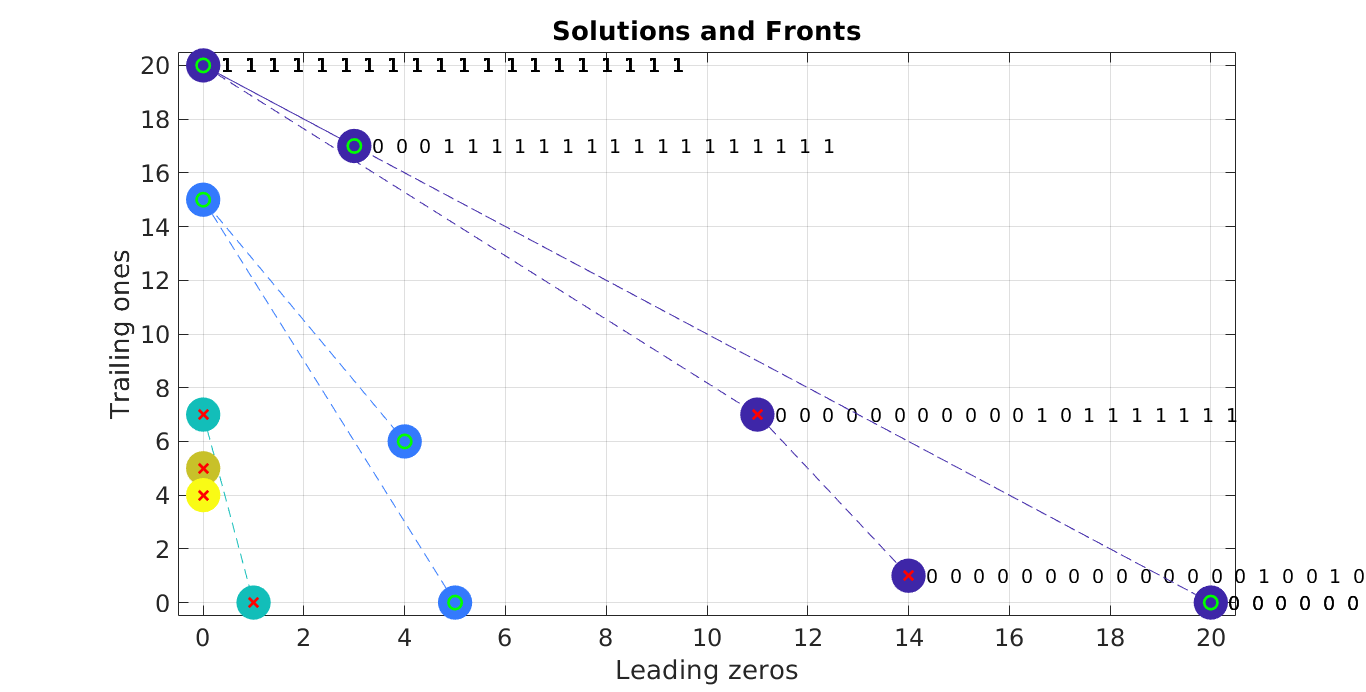
\includegraphics[width=\textwidth]{1000_gen_10_pop.png}
				\end{center}
				\caption{Population size = 10, while number of generations = 1000}
				\label{figure2}
			\end{figure}
			
	 \textbf{Answer}: For the case when the algorithm is set with population size of 10 and number of generations 1000 (second scenario - figure \ref{figure2}), the algorithm finds  optimal solutions in some generations, but not all found optimal solutions are kept until the end of algorithm's run. This is due to fact that the space for exploration is very small compared to the another case. Here, some optimal solutions get "destroyed" over time, i.e. in this case, the algorithm performs much more of exploitation, rather than exploration. However, in the first scenario the population size is 100 (figure \ref{figure1}) and now the algorithm has the chance to explore bigger solution space and thus converge with more optimal solutions.
	\item (5pts) Imagine you were to replace the objective of ``leading zeros'' with ``largest binary number''. Predict the result, and give your reasoning.\\ [2mm]
	\textbf{Answer}: With the ``largest binary number'' objective function, the algorithm would  converge to the single solution, i.e. solution string that contains all ones. The reason for this is the fact that as we add more ones to the bit string, its value becomes bigger and this satisfies both objective functions.
	\item (5pts) Imagine you were to add a third objective: ``non-consecutive ones and zeros'' (ones not touching ones and zeros not touching zeros, e.g. 0101 and 1010 are the most optimal 4 bit solutions). How would you adjust the hyperparameters to get a satisfactory result?
	\item (5pts) In many GAs and ESs populations must be ranked, but no special methods are used. Why is a faster sort in MOO so important?
\end{itemize}

\newpage
\subsection{** Extra Credit ** (+ 10pts in examination)}
Implement the third objective ``non-consecutive ones and zeros''
\begin{enumerate}
	\item How many non-dominated solutions are possible? (Hint: start with a smaller length and test)
	\item What changes did you make to the algorithm and hyperparameters to get a good result?
	\item List the solutions in your 1st front. Are they all Pareto optimal? How complete is your front (in percentage, based on $\#1$)
	\item Plot the end result in 3D. (Use \mcode{plot3} or \mcode{scatter3})
\end{enumerate}


\end{document}














